There are some research groups working on braille display system based on dielectric elastomer \cite{qu_refreshable_2021}.
Dielectric elastomer is an electroactive polymer that can produce large deformation under the electric field and return to its original size immediately after the electric field being removed.
This perfectly satisfies the requirement for making a refreshable braille display.
However, this mechanism is strongly dependent on high voltage (HV) supplies and may pose potential dangers to the human body.
Although one of the groups suggested using Triboelectric nanogenerators (TENGs) as safer HV supply, we still have to give it up because of the excessive cost and difficulty accessing the same material. 
\todo[inline]{Paragraph above needs some strong work. What's the point of the picture associated with this paragraph?}

\begin{figure}[h]\centering
    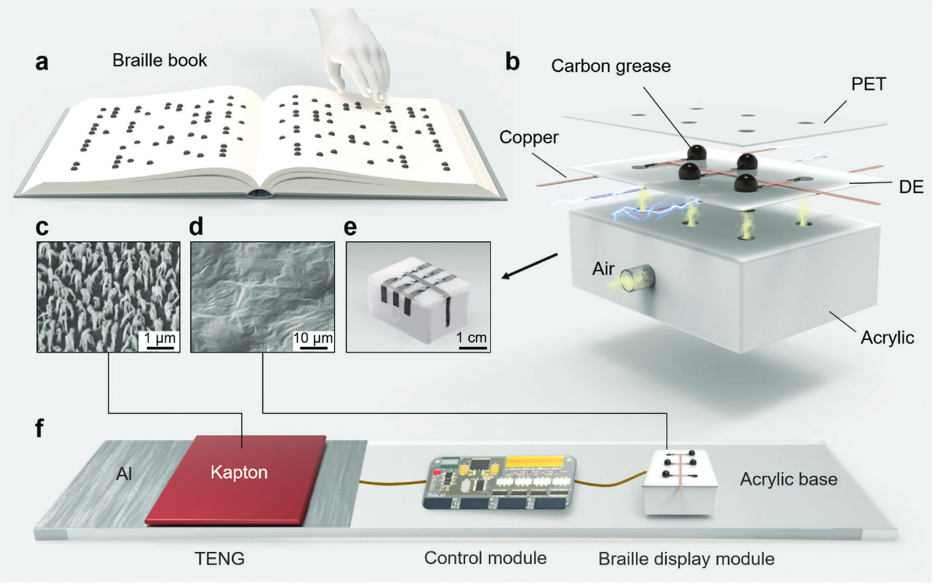
\includegraphics[width=0.7\textwidth]{figures/teng.png}
    \caption[Dielectric elastomer Braille display]{Design of the refreshable Braille display system. a) Schematic diagram of a conventional Braille book. b) Exploded view of the Braille display module. c) SEM image of nanostructure on the surface of Kapton film treated by ICP reactive-ion etching. d) SEM image of the carbon grease on the DED. e) Photo of the Braille display module. f) Schematic diagram of the RBDS with control module \cite{qu_refreshable_2021}.}
    \label{fig:teng.png}
\end{figure}

Two cheap mechanisms that rely on heat were investigated, but quickly discarded due to high operational temperatures and required times to cool down:

\paragraph{Shaped Memory Alloy (SMA)}
Shown in figure \ref{fig:sma}, have the ability to be shaped when cold and return to their predefined original position when heated and thus being a potential solution for actuators in the braille display system \cite{chaves_microtuators_2009}.

\begin{figure}[h]\centering
    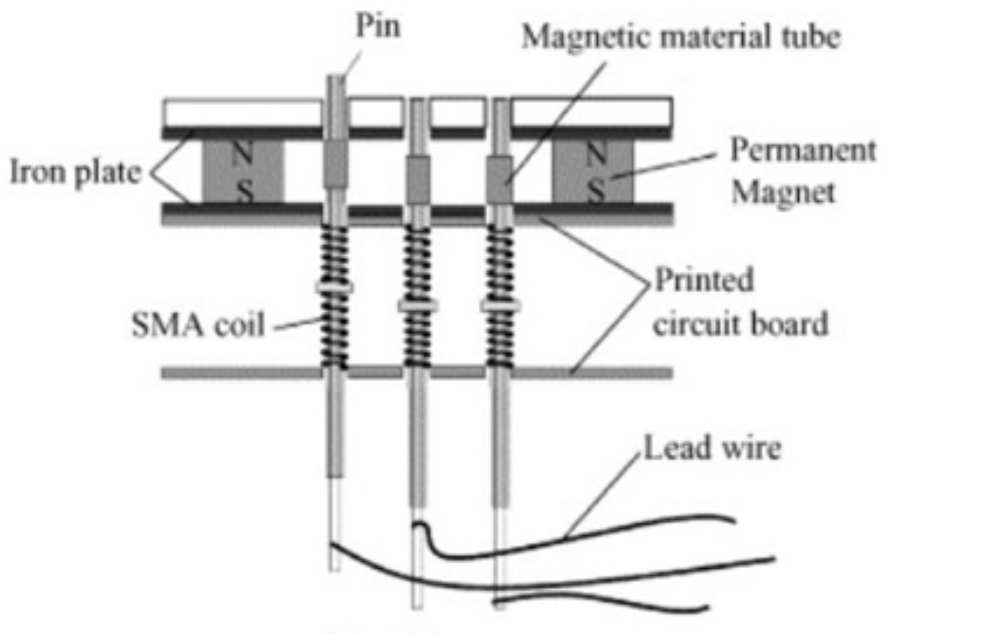
\includegraphics[width=0.5\textwidth]{figures/Coil_SMA_mechanism.png}
    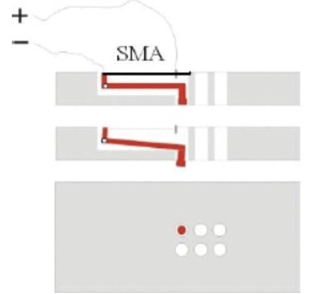
\includegraphics[height=5cm]{figures/sma-mechanism.png}
    \caption[Schematics of Shaped Memory Alloy (SMA) mechanisms]{ a) Schematic model of the SMA coil microactuator b) Schematic model of the SMA wire microactuator with lever \cite{haga_dynamic_2005}.}
    \label{fig:sma}
\end{figure}
\todo[]{Fix these figures. Caption doesn't match numbering system}

\paragraph{Paraffin wax}
Shown in figure \ref{fig:paraffin}, can also act as the actuators \cite{lee_micromachined_2005}. When paraffin wax is heated, it expands.
The system utilizes the air pressure caused by this expansion to push a mebrane diaphragm up to generate the dots.

\begin{figure}[h] \centering
    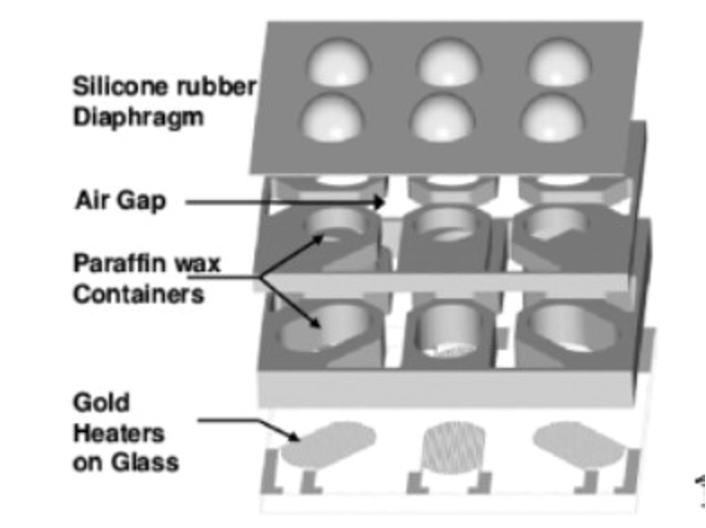
\includegraphics[width=0.5\textwidth]{figures/paraffin.png}
\caption[Paraffin-based Braille cell]{Exploded view of paraffin wax-based Braille cell design \cite{lee_micromachined_2005}.}
\label{fig:paraffin}
\end{figure}
